\documentclass[12pt,a4paper]{article}
\usepackage[utf8]{inputenc}
\usepackage[german]{babel}
\usepackage[T1]{fontenc}
\usepackage{amsmath}
\usepackage{amsfonts}
\usepackage{amssymb}
\usepackage{graphicx}
\usepackage{siunitx}
\usepackage{float}
\usepackage[left=2cm,right=2cm,top=2cm,bottom=2cm]{geometry}
\author{Gerald}

\begin{document}
\sisetup{separate-uncertainty = true}
	\setlength{\parindent}{0pt} 
	\begin{center}
		{\LARGE Versuchsprotokoll}\\
		\begin{large}
			zum Fortgeschrittenenpraktikum im Bachelorstudiengang Physik\\[0.4cm]
			an der RWTH Aachen\\
			II. Physikalisches Institut A\\[5.5cm]
			\Large\textbf{\textsl{Rastertunnelmikroskopie (STM)}}\\[5.5cm]
			\normalsize\textit{vorgelegt\\von}\\[0.4cm]
			\large{Moritz Berger (355244)\\Gerald Kolter (355005)}\\Gruppe 30\\[2cm]
			\large \textbf{Wintersemester 2017/18}
		\end{large}
	\end{center}
	\newpage
	
	\tableofcontents
	\newpage

\section{Versuchsziel}
Das Ziel des Versuchs besteht darin, mit einem Rastertunnelmikroskop bei der Vermessung einer Goldprobe die Auswirkung der Einstellungen auf das Messergebnis zu untersuchen. Mit einer Probe eines hochorientierten pyrolytischen Graphit (HOPG) wird der Abstand der Gitterebenen bestimmt und eine Kalibration in x- und y-Richtung durchgeführt.

\section{Aufbau}
Das verwendete Rastertunnelmikroskop besteht aus einem Halter für die Platin-Iridium-Spitze, der mit piezoelektrischen Kristallen in allen drei Raumrichtungen bewegt werden kann, und einem Probenhalter, der auf einem sogenannten Schrittmotorantrieb liegt. Dieser funktioniert ebenfalls mit einem piezoelektrischen Kristall und dient lediglich der Grobannäherung. Spitze und Probe sind über eine Spannungsquelle verbunden, wobei gleichzeitig der in diesem Kreis fließende Strom gemessen wird. Dieser Strom kommt bei kleinen Abständen zwischen Spitze und Probe durch den Tunneleffekt zustande. Die Abhängigkeit zwischen Strom und Abstand ist exponentiell und damit sehr stark.\\
Die Spitze wird mit den piezoelektrischen Kristallen über die Probe gerastert, wobei jede Linie in x-Richtung vorwärts und rückwärts abgefahren wird.\\
Eine Regelungselektronik steuert die z-Richtung der Spitze in Abhängigkeit des Tunnelstroms. Dabei gibt der sogenannte I-Gain an, wie schnell die Regelung auf kurze Pulse reagiert.



%\begin{figure}
%\centering
%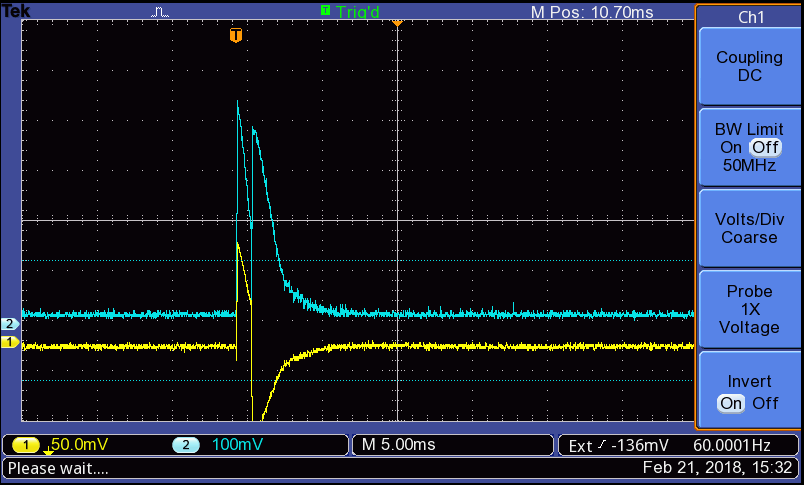
\includegraphics[scale=0.8]{Bilder/F0003TEK.PNG}
%\caption{Ergebnis einer einzelnen Messung zur Bestimmung von T1. Die blaue Kurve zeigt das zu untersuchende Signal.}
%\label{fig:MessungT1_Beispiel}
%\end{figure}



\section{Durchführung}
\subsection{Untersuchung der Mikroskopeigenschaften mit einer Goldprobe}

\begin{table}
\centering
\begin{tabular}{|c|c|}
\hline 
Bereichgröße & (75,23 nm)$^2$ \\ 
\hline 
Zeit pro Linie & 0,2 s \\
\hline 
Tunnelspannung & 450 mV \\ 
\hline 
Messpunkte pro Linie & 256 \\
\hline 
Sollwert Tunnelstrom & 1 nA \\
\hline 
\end{tabular} 
\caption{Einstellungen der Messparameter bei Vermessung der Goldprobe. Bei dieser Messreihe wurde der IGain zwischen 1000 und 11000 verändert.}
\label{tab:IGain_Einstellungen}
\end{table}

Für die Untersuchung der Empfindlichkeit der Einstellparameter wird auf der Goldprobe zunächst ein Bereich mit markanter Struktur gesucht. Dieser Bereich wird für vier verschiedene Werte für den I-Gain bei ansonsten gleichbleibenden Parametern vermessen. Diese Einstellungen sind in Tabelle \ref{tab:IGain_Einstellungen} eingetragen.\\
In einer zweiten Messreihe wird erneut ein Bereich mit markanter Struktur vermessen, wobei anstelle des I-Gain die Messzeit pro Zeile verändert wird. Für den I-Gain wurde hierbei der Wert, der sich in der ersten Messreihe als beste Annäherung des Idealwertes herausgestellt hat, verwendet (I-Gain = 3000). Alle anderen Parameter blieben unverändert.

\subsection{Untersuchung von HOPG}

\section{Ergebnisse}
\subsection{Untersuchung der Mikroskopeigenschaften mit einer Goldprobe}

\subsection{Untersuchung von HOPG}

\section{Fazit}

\section{Anhang}


\end{document}